\documentclass[10pt,oneside]{article}

%%%%%%%%%%%%%
\setlength{\textheight}{8.75in} %Letter is 11in, less 2 for margins, less 0.25 for footer
\setlength{\oddsidemargin}{0.0in} %gets +1inc
\setlength{\evensidemargin}{0.0in} %gets +1inch
\setlength{\textwidth}{6.50in} %Letter is 8.5, less 2 inches for margins
\setlength{\topmargin}{0.5in}
\setlength{\headheight}{0in}
\setlength{\headsep}{0in}
\setlength{\parindent}{0.25in}
%%%%%%%%%%%%

% use letters instead of symbols to accommodate >7 authors
\makeatletter
\let\@fnsymbol\@alph
\makeatother

\usepackage[utf8]{inputenc}
\usepackage[numbers]{natbib}
\usepackage{graphicx}
\usepackage[colorlinks=true,citecolor=black,urlcolor=blue]{hyperref}

\title{%Hack to get the logo on the PDF front page:
\vspace{-1.5in}

\includegraphics[width=0.4\textwidth]{../presentation/figures/biopython.jpg} \\
\vspace{3mm}Biopython Project Update 2017}
\author{
	\underline{Sourav Singh}\thanks{Dept. of Computer Engineering, VIIT, Pune, India. Email: \href{mailto:ssouravsingh12@gmail.com}{ssouravsingh12@gmail.com}},
    Christian Brueffer\thanks{Department of Clinical Sciences, Lund University, Lund, SE},
    Peter Cock\thanks{Information and Computational Sciences, James Hutton Institute, Invergowrie, Dundee, UK},\\
    and the Biopython Contributors\thanks{See \href{https://github.com/biopython/biopython/blob/master/CONTRIB.rst}{contributor listing on GitHub}.}}
\date{18\textsuperscript{th} Bioinformatics Open Source Conference (BOSC) 2017, Prague, CZ}

\begin{document}
\maketitle
\thispagestyle{empty}

\vspace{-0.2in}
\noindent
Website: \url{http://biopython.org} \\
Repository: \url{https://github.com/biopython/biopython} \\
License: Biopython License Agreement (BSD like, see \url{http://www.biopython.org/DIST/LICENSE}) \\

The Biopython Project is a long-running distributed collaborative effort,
supported by the Open Bioinformatics Foundation, which develops a freely
available Python library for biological computation \cite{AppNote}.
We present here details of the Biopython releases since BOSC 2016,
namely Biopython 1.68, 1.69 and 1.70. Together these had 82 named
contributors including 51 newcomers which reflects our policy of
trying to encourage even small contributions.

Biopython 1.68 (August 2016) was a relatively small release,
with the main new feature being support for RSSB's new binary
Macromolecular Transmission Format (MMTF) for structural data.

Biopython 1.69 (April 2017) represents the start of our re-licensing plan, to transition away
from our liberal but unique \emph{Biopython License Agreement} to the similar
but very widely used \emph{3-Clause BSD License}. We are reviewing the code
base authorship file-by-file, in order to gradually dual license the entire
project.

Major new features include: a new parser for the ExPASy Cellosaurus cell line
database, catalogue and ontology; support for the UCSC Multiple Alignment Format (MAF),
FSA sequencing files, version 4 of the Affymetrix CEL format; updates to the
REBASE February 2017 restriction enzyme list;
Bio.PDB.PDBList now can download more formats including MMTF;
enhanced PyPy support by taking advantage of NumPy and compiling most of the Biopython C code modules.

Biopython 1.70 (July 2017) has internal changes to better support the
now standard \verb|pip| tool for Python package installation.
Major new features include:
support for Mauve's eXtended Multi-FastA (XMFA) file format,
updates to our BLAST XML and MEME parsers, ExPASy support,
and phylogenetic distance matrices.
This release is noteworthy for our new logo (below),
contributed by Patrick Kunzmann. This draws on our original double helix logo
(above), and the blue and yellow colors of the current Python logo:

\begin{center}
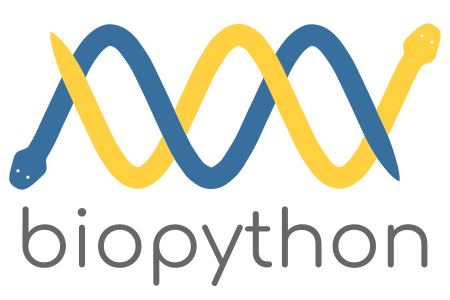
\includegraphics[height=2.5cm]{../presentation/figures/biopython_logo_s.png}
\end{center}

All releases fixed miscellaneous bugs, enhanced the test suite,
and continued efforts to follow the PEP8 and PEP257 coding style guidelines
which is now checked automatically with GitHub-integrated continuous integration
testing using TravisCI.
We now also use AppVeyor for continuous integration testing under Windows.
Current efforts include improving the unit test coverage, which is easily viewed
online at \href{https://codecov.io/github/biopython/biopython/}{CodeCov.io}.

\begin{thebibliography}{}

\bibitem[Cock {\it et al}., 2009]{AppNote}Cock, P.J.A., Antao, T., Chang, J.T., Chapman, B.A., Cox, C.J., Dalke, A., Friedberg, I., Hamelryck, T., Kauff, F., Wilczynski, B., de Hoon, M.J. (2009) Biopython: freely available Python tools for computational molecular biology and bioinformatics. {\it Bioinformatics} {\bf 25}(11) 1422-3. \href{http://dx.doi.org/10.1093/bioinformatics/btp163}{doi:10.1093/bioinformatics/btp163}

\end{thebibliography}

\end{document}
